\documentclass[aps,prd,twocolumn,amsmath,amssymb,nofootinbib]{revtex4-2}

\usepackage[T1]{fontenc}
\usepackage[utf8]{inputenc}
\usepackage{mathtools}
\usepackage{xcolor}
\usepackage{tikz}
\usetikzlibrary{arrows.meta,calc}
\usepackage{hyperref}
\usepackage{orcidlink}
\hypersetup{
  colorlinks=true,
  linkcolor=blue!55!black,
  citecolor=blue!55!black,
  urlcolor=blue!55!black,
  pdfauthor={Karl Svozil},
  pdftitle={Operationalizing a Spacetime Hole},
  pdfsubject={Traversal cost, defects, repulsion, and connectivity}
}

\newcommand{\dd}{\mathrm{d}}
\newcommand{\eff}{\mathrm{eff}}
\newcommand{\opt}{\mathrm{opt}}
\newcommand{\BY}{\mathrm{BY}}
\DeclareMathOperator{\erf}{erf}

\begin{document}

\title{Operationalizing a Spacetime Hole:
\texorpdfstring{\\\large}{ }Traversal Cost, Defects, Repulsion, and Connectivity}
\author{Karl Svozil\,\orcidlink{0000-0001-6554-2802}}
\affiliation{Institute for Theoretical Physics,
Vienna University of Technology (TU Wien),
Wiedner Hauptstrasse 8--10/136, 1040 Vienna, Austria}
\date{14 July 2026}

\begin{abstract}
The phrase ``a hole in spacetime'' conflates four operationally distinct
questions concerning curvature, force, traversal cost, and connectivity.  We
make the intuition of ``less to traverse'' precise through a
reference-relative boundary kernel $E_U$: the difference in earliest reception
time between a region and a reference filling with the same calibrated
boundary.  In a static spacetime, light probes the optical metric
$h_{ij}/N^2$, massive trajectories probe an energy-dependent Jacobi metric,
and propulsive effort remains protocol dependent.  A regularized surplus-angle
cone has negative curvature and increased transverse optical cost but unchanged
radial cost and no ordinary radial force, showing that curvature sign alone
does not diagnose a shortcut.  By contrast, a spherical thin shell with a
negative Schwarzschild exterior contracts the optical metric and produces a
Shapiro advance, demagnification, and composition-independent outward free
fall.  The shell requires exotic surface stress and presents an energy barrier
to inward-moving massive particles.  Its four-volume form nevertheless equals
the flat expression in areal coordinates, so volume density is not the
controlling traversal observable.  Deleting a region while holding the metric
cost fixed cannot produce a shortcut: an advance requires a lower path cost,
an enlarged path set, or both.  We conclude with coarse-grained and
multispecies tests for a universal effective geometry and a six-item reporting
checklist.
\end{abstract}

\maketitle

\section{Introduction: operational questions behind the metaphor}
\label{sec:introduction}

The phrase ``a hole in spacetime'' is evocative but underspecified.  It may
suggest missing microscopic constituents, reduced spatial volume, negative
curvature, repulsive free fall, an early-arriving signal, an excised region, or
a bridge between otherwise distant locations.  None of these meanings implies
the others automatically.  The purpose of this paper is to separate the
operational content of the metaphor from associations supplied by an external
picture of the manifold.

An embedded observer instead works with coincidences of events, causal order,
calibrated clocks and volumes, signal responses, and the motion of test bodies~\cite{toffoli:79,svozil-94}.
The intuition pursued here concerns the time or effort needed to traverse a
region.  Its closest geometric realization is not a scalar density of
spacetime but a cost assigned to directions and paths relative to a specified
reference.  For light in a static spacetime this cost is encoded exactly by the
optical metric.  For massive particles it also depends on energy.  ``Effort''
is more protocol dependent still: free fall costs no proper acceleration,
whereas hovering, prescribed transit time, and rocket fuel define different
functionals.

It is therefore useful to ask four questions separately.  Do neighboring paths
spread?  Are freely falling bodies pushed?  What does an existing route cost?
And which routes exist in the first place?  Table~\ref{tab:fourquestions}
associates each question with its natural measurements.

\begin{table*}[ht]
\centering
\begin{ruledtabular}
\begin{tabular}{llll}
Question & Operational observable & Geometric structure & Does not determine \\
\hline
Do paths spread? & circumference ratios, lensing & curvature, angle, holonomy & force or travel time \\
Are bodies pushed? & released-body acceleration, redshift & lapse gradient $\nabla N$ & topology \\
What does a route cost? & arrival-time kernel, energy threshold & optical or Jacobi metric & curvature sign \\
Which routes exist? & path classes, images, bridges & connectivity, topology & local force or cost
\end{tabular}
\end{ruledtabular}
\caption{Four operational questions contained in the word ``hole.''  The
entries are deliberately nonexclusive: for example the lapse contributes to
both redshift and optical cost, but neither observable fixes the other sectors
without additional information.}
\label{tab:fourquestions}
\end{table*}

The separation also resolves an ambiguity in the word \emph{shortcut}.
Earlier arrival is an outcome.  Lower metric cost and changed connectivity are
distinct mechanisms that can produce it.

The remainder of the paper is organized as follows.
Section~\ref{sec:boundary} defines the reference-relative boundary kernel.
Sections~\ref{sec:optical} and \ref{sec:massive} formulate null and massive
traversal costs, respectively.  Sections~\ref{sec:defects} and \ref{sec:lapse}
separate angle defects from lapse-driven repulsion, and
Sec.~\ref{sec:shell} supplies an exact thin-shell realization.
Section~\ref{sec:connectivity} proves that excision at fixed cost cannot create
a shortcut.  Sections~\ref{sec:microscopic} and \ref{sec:universality} state
the conditions under which microscopic or coarse-grained data can support a
universal effective geometry.  Section~\ref{sec:discussion} compares the
measurement protocols and relevant scales, and Sec.~\ref{sec:conclusion}
summarizes the operational conclusions.

\section{Boundary data and a reference-relative kernel}
\label{sec:boundary}

An observer confined to spacetime has access to coincidences of events, causal
order, clock readings, freely falling bodies, signal responses, and volume
measurements.  At resolution $\epsilon$ we summarize these data schematically
as
\begin{equation}
 \bigl(X_{\epsilon},\preceq_{\epsilon},\tau_{\epsilon},
 \nu_{\epsilon},\{\mathcal R_{\epsilon,a}\}\bigr),
\end{equation}
where $a$ labels probe species or channels.  Under standard causality
hypotheses, causal relations determine the conformal geometry, while calibrated
volume data determine its remaining scale
\cite{Malament-1977,hawking-king-mccarthy-1976}.  At finite resolution it is
safer, however, to state claims directly in terms of measured boundary data.

Let a world tube $B$ of calibrated emitters, receivers, and clocks surround a
region $U$.  For a specified channel and protocol, let
$\mathcal T_U(b_1,b_2)$ be the infimum of reception times over all admissible
signals from $b_1$ to $b_2$.  Multiple images are included, and caustics are
resolved by the protocol.  Choose a specified reference filling $U_0$, not
necessarily flat, together with a fixed boundary isometry
$\iota:B_0\rightarrow B$ that identifies emitters, receivers, the induced
boundary metric, clock calibration, and emission prescription.  A flat
reference is used only when it is compatible with these boundary data.  The
boundary time is proper time, $\dd\tau_B=N_B\dd t$; the same $N_B$ is used in
both fillings and may conventionally be normalized to unity.  We then define
\begin{equation}
 E_U(b_1,b_2)
 =c\,[\mathcal T_U(b_1,b_2)-\mathcal T_{U_0}(b_1,b_2)].
 \label{eq:kernel}
\end{equation}
Thus $E_U>0$ is a delay, $E_U<0$ an advance, and $E_U=0$ neutrality in that
channel.  This kernel is the primary operational meaning of more or less to
traverse.  It does not require an arbitrary point-by-point identification of
the two interiors.  It is invariant under interior coordinate changes but
depends, as every relative observable must, on the chosen pair $(U_0,\iota)$.

\section{Null traversal cost: the optical metric}
\label{sec:optical}

Consider a static spacetime
\begin{equation}
 \dd s^2=-N(\boldsymbol{x})^2c^2\dd t^2
 +h_{ij}(\boldsymbol{x})\dd x^i\dd x^j,
 \qquad N>0,
 \label{eq:staticmetric}
\end{equation}
with the time normalization fixed at the comparison boundary.  This fixing is
essential: under $t'=\alpha t$ one has $N'=N/\alpha$ and
$h^{\opt\prime}_{ij}=\alpha^2h^{\opt}_{ij}$.  Once the same boundary proper
time has been chosen in the physical and reference fillings, the optical
comparison is unambiguous.  Along a null curve,
\begin{equation}
 c\,\dd t
 =\frac{\sqrt{h_{ij}\dd x^i\dd x^j}}{N}
 =\sqrt{h^{\opt}_{ij}\dd x^i\dd x^j},
 \qquad h^{\opt}_{ij}=\frac{h_{ij}}{N^2}.
 \label{eq:opticalmetric}
\end{equation}
The spatial projections of light rays are stationary curves of this optical
length, and the earliest admissible ray realizes its infimum under the stated
boundary protocol \cite{perlick-1990-ii,gibbons-werner-2008}:
\begin{equation}
 \mathcal T_U(b_1,b_2)
 =\frac{1}{c}\inf_{\gamma:b_1\rightarrow b_2}
 \int_{\gamma}\sqrt{h^{\opt}_{ij}\dd x^i\dd x^j}.
 \label{eq:fermat}
\end{equation}
Because $\dd t=\dd\tau_B/N_B$ at the receiver network, the infimum in
Eq.~\eqref{eq:fermat} is directly the earliest boundary-clock reading after the
fixed normalization.  Every local freely falling observer still measures the
vacuum speed of light to be $c$.  An advance is a global comparison of optical
lengths and boundary clocks, not a local superluminal speed.

If a map between the reference interiors has additionally been chosen, a
directional cost ratio can be defined by
\begin{equation}
 \eta_{\rm dir}(x,v)=
 \frac{\sqrt{h_{ij}v^iv^j}/N}
 {\sqrt{h^{(0)}_{ij}v^iv^j}/N_0}.
 \label{eq:directionalcost}
\end{equation}
Then $\eta_{\rm dir}<1$ means less optical cost in direction $v$.  A scalar
geometric-mean proxy in three spatial dimensions is
\begin{equation}
 \eta_{\rm vol}^{\opt}
 =\left(\frac{\det h^{\opt}}{\det h^{\opt}_0}\right)^{1/6},
 \label{eq:optvolproxy}
\end{equation}
but it hides anisotropy: its value can be below unity even when some
directions cost more.  The full quadratic form, or ultimately the boundary
kernel \eqref{eq:kernel}, is more informative.

In a weak, approximately isotropic field,
\begin{equation}
 \dd s^2\simeq
 -\left(1+\frac{2\Phi}{c^2}\right)c^2\dd t^2
 +\left(1-\frac{2\gamma\Phi}{c^2}\right)\dd\boldsymbol{x}^2,
\end{equation}
so the directional optical cost relative to the coordinate reference is
\begin{equation}
 \eta_{\rm dir}\simeq
 1-\frac{(1+\gamma)\Phi}{c^2}.
 \label{eq:weakopticalcost}
\end{equation}
With the convention $\Phi=-GM/r$ for ordinary positive mass, this is a delay.
A positive potential perturbation, as produced by the negative-mass toy model
below, instead gives an advance.  This is the limited sense in which a
refractive-index analogy is useful; it should not be promoted to a fundamental
medium without tests of dispersion and universality.

\section{Massive particles: time, access, and effort}
\label{sec:massive}

For a freely falling particle of rest mass $m$ and conserved Killing energy
$E$ in \eqref{eq:staticmetric}, the spatial trajectory at fixed $E$ is governed
by the Jacobi metric \cite{gibbons-2016-jacobi}
\begin{equation}
 j^{(E)}_{ij}
 =\frac{E^2-m^2c^4N^2}{c^2N^2}\,h_{ij}.
 \label{eq:jacobimetric}
\end{equation}
It exists only where
\begin{equation}
 E\geq mc^2N.
 \label{eq:accesscondition}
\end{equation}
Unlike the null optical metric, $j^{(E)}_{ij}$ is energy dependent.  Different
massive beams can therefore assign different effective traversal structures to
the same spacetime even when all follow one spacetime metric.

Propulsive effort is a further observable, not another name for geodesic
length.  One possible protocol assigns a prescribed worldline $\Gamma$ the
integrated proper acceleration
\begin{equation}
 \mathcal A[\Gamma]=
 \int_{\Gamma}\sqrt{a_{\mu}a^{\mu}}\,\dd\tau,
 \label{eq:properacccost}
\end{equation}
but fuel use also depends on the vehicle, exhaust velocity, payload, and speed
profile.  Free fall has $\mathcal A=0$ whether the trip is long or short.
Consequently ``less time'' and ``less effort'' should be reported as separate,
protocol-labelled quantities.

\section{Angle defects do not measure depletion}
\label{sec:defects}

The geometric theory of crystal defects provides a more specific
continuum-mechanical realization: disclinations carry curvature, whereas
dislocations carry torsion.  In the Volterra construction, removing or
inserting an angular sector produces the conical geometry considered here
\cite{kleinert-2000}.  Remove a wedge from a disk and glue its edges, or insert
a wedge and glue.  Outside the core,
\begin{equation}
 h_{\beta}=\dd r^2+\beta^2r^2\dd\phi^2,
 \qquad 0\leq\phi<2\pi.
 \label{eq:cone}
\end{equation}
For $\beta<1$ the circumference $2\pi\beta r$ has a deficit; for $\beta>1$
it has a surplus.  The curvature concentrated at the apex has total weight
\begin{equation}
 \int K\,\dd A=2\pi(1-\beta).
 \label{eq:conecurvature}
\end{equation}

A smooth core of radius $a$ is obtained from
\begin{align}
 h&=\dd r^2+b(r)^2\dd\phi^2,\nonumber\\
 b(r)&=r+(\beta-1)\left[
 r-\frac{\sqrt{\pi}a}{2}\erf\left(\frac{r}{a}\right)
 \right].
 \label{eq:smoothcone}
\end{align}
Here $b'(0)=1$, $b'(\infty)=\beta$, and
\begin{equation}
 K(r)=-\frac{b''(r)}{b(r)}<0
 \quad (r>0,\ \beta>1).
 \label{eq:smoothconecurvature}
\end{equation}
The integrated curvature remains $2\pi(1-\beta)$ because
$\int K\,\dd A=-2\pi[b'(\infty)-b'(0)]$; it is independent of the regulator
size $a$.  The defect charge is therefore conserved while its curvature
density is smeared.  For $\beta\neq1$ the geometry is asymptotically conical,
so comparisons with Euclidean space must be made at a specified boundary and
with an explicit reference subtraction.

The traversal interpretation now gives a sharp result.  When $N=1$, the
optical metric equals \eqref{eq:cone}.  Radial cost is exactly $\dd r$, whereas
angular cost is $\beta r\dd\phi$.  A surplus defect has negative curvature but
\emph{more} transverse cost; a deficit has less transverse cost but positive
concentrated curvature.  Curvature sign is therefore not a density of what a
ray must traverse.

In the static cylindrical extension
\begin{equation}
 \dd s^2=-N(r)^2c^2\dd t^2+\dd r^2+b(r)^2\dd\phi^2+\dd z^2,
 \label{eq:cylmetric}
\end{equation}
an ideal cone with $N=1$ is locally flat away from the axis.  It has global
holonomy and lensing-like effects, as for cosmic strings
\cite{vilenkin-1981}, but no ordinary local radial force.  In $2+1$ Einstein
gravity this distinction is exact: source-free regions are flat and localized
sources act through global conical geometry \cite{deser-jackiw-thooft-1984}.

\section{Repulsion requires a lapse gradient}
\label{sec:lapse}

In the weak-field limit,
\begin{equation}
 N^2=1+\frac{2\Phi}{c^2},
 \qquad \ddot{\boldsymbol{x}}\simeq-\boldsymbol{\nabla}\Phi.
 \label{eq:newtonianlimit}
\end{equation}
A smooth positive hump
\begin{equation}
 \Phi(r)=\frac{\Phi_0a}{\sqrt{r^2+a^2}},
 \qquad \Phi_0>0,
 \label{eq:potentialhump}
\end{equation}
gives
\begin{equation}
 -\partial_r\Phi
 =\frac{\Phi_0ar}{(r^2+a^2)^{3/2}}>0.
 \label{eq:outwardacc}
\end{equation}
It simultaneously lowers weak-field optical cost through
\eqref{eq:weakopticalcost}.  The force and the advance arise from related but
different combinations of metric components: slow free fall probes a lapse
gradient, while null travel probes $h_{ij}/N^2$.

Equations \eqref{eq:cylmetric}--\eqref{eq:potentialhump} are kinematic until
their effective stress tensor
\begin{equation}
 T^{\eff}_{\mu\nu}=\frac{c^4}{8\pi G}G_{\mu\nu}[g]
\end{equation}
has been computed and tested.  Negative spatial curvature cannot replace this
dynamical calculation.  For complete asymptotically flat data satisfying the
appropriate energy conditions, positive-mass results impose strong
restrictions on isolated negative total mass \cite{schoen-yau-1979}.  A
background-relative underdensity or a compensated construction is therefore
more conservative than an isolated negative-mass object.

\section{Exact realization: a repulsive thin shell}
\label{sec:shell}

We now set $c=1$.  Take a flat interior with time $T$,
\begin{equation}
 \dd s^2_-=-\dd T^2+\dd r^2+r^2\dd\Omega^2,
 \qquad r<a,
 \label{eq:interior}
\end{equation}
and a Schwarzschild exterior with time $t$,
\begin{equation}
 \begin{aligned}
  \dd s^2_+&=-f(r)\dd t^2+f(r)^{-1}\dd r^2
               +r^2\dd\Omega^2,\\
  f(r)&=1-\frac{2GM}{r},\qquad r>a.
 \end{aligned}
 \label{eq:exterior}
\end{equation}
Let $M=-|M|$, so
\begin{equation}
 f(r)=1+\frac{2G|M|}{r}>1.
 \label{eq:negativef}
\end{equation}
The shell $\Sigma$ is $r=a$ with proper time $\tau$.  Continuity of its
induced metric requires
\begin{equation}
 \dd T=\dd\tau,
 \qquad
 \dd t=\frac{\dd\tau}{\sqrt{f(a)}},
 \qquad
 \dd s^2_{\Sigma}=-\dd\tau^2+a^2\dd\Omega^2.
 \label{eq:matching}
\end{equation}

Choose the unit normal to point toward increasing $r$ and use
$K_{ab}=-n_{\mu}\nabla_a e^{\mu}{}_b$.  The nonzero mixed components are
\begin{align}
 K^-{}^{\tau}{}_{\tau}&=0,
 &K^-{}^{\theta}{}_{\theta}=K^-{}^{\phi}{}_{\phi}&=\frac{1}{a},
 \label{eq:Kminus}\\
 K^+{}^{\tau}{}_{\tau}&=\frac{GM}{a^2\sqrt{f(a)}},
 &K^+{}^{\theta}{}_{\theta}=K^+{}^{\phi}{}_{\phi}
 &=\frac{\sqrt{f(a)}}{a}.
 \label{eq:Kplus}
\end{align}
With
\begin{equation}
 S^a{}_b=\frac{1}{8\pi G}
 \left([K]\delta^a{}_b-[K^a{}_b]\right),
 \label{eq:israel}
\end{equation}
the Israel junction conditions \cite{israel-1966,poisson-2004} give
\begin{equation}
 \sigma\equiv-S^{\tau}{}_{\tau}
 =\frac{1}{4\pi Ga}
 \left(1-\sqrt{1+\frac{2G|M|}{a}}\right)<0,
 \label{eq:sigma}
\end{equation}
and
\begin{equation}
 p\equiv S^{\theta}{}_{\theta}
 =\frac{1}{8\pi Ga}
 \left[
 \frac{1+G|M|/a}{\sqrt{1+2G|M|/a}}-1
 \right]>0.
 \label{eq:pressure}
\end{equation}
The induced $2+1$ surface stress tensor violates all of the standard
pointwise surface energy conditions: $\sigma+p<0$ violates the null condition,
$\sigma<0$ violates the weak and dominant conditions, and the strong condition
also fails.  The shell is therefore an effective exotic source, not a proposal
for ordinary matter.  These signs do not by themselves settle radial
stability.  The radial shell potential depends on the equation of state; in
particular, without specifying the perturbative response
$\delta p/\delta\sigma$, neither stability nor instability follows.

\subsection{Force and massive-particle access}

Static exterior observers have four-velocity $u=f^{-1/2}\partial_t$.  Their
acceleration is
\begin{equation}
 a_r=\partial_r\ln\sqrt f=\frac{GM}{r^2f},
 \qquad
 a^r=\frac{GM}{r^2}.
 \label{eq:staticacc}
\end{equation}
For $M<0$, hovering requires inward proper acceleration; a released body moves
outward.  The effect is composition independent because all test bodies follow
the same metric geodesics.

Timelike geodesics, written in terms of specific energy $\mathcal E$ and
specific angular momentum $\ell$, satisfy
\begin{equation}
 \dot r^2+V_{\eff}(r)=\mathcal E^2,
 \qquad
 V_{\eff}=f(r)\left(1+\frac{\ell^2}{r^2}\right).
 \label{eq:timelikepotential}
\end{equation}
This potential decreases monotonically toward its asymptotic value as $r$
increases, so there are no circular timelike geodesics in the exterior.  The
access condition \eqref{eq:accesscondition} also exposes the difference
between time and effort: since $N=\sqrt f>1$, a particle released from rest at
infinity has $\mathcal E=1$ (equivalently physical energy $E_{\rm phys}=m$)
and cannot penetrate to finite $r$.  Inward traversal needs
additional kinetic or propulsive energy even though the null route is
optically shorter.  Outward traversal, by contrast, is assisted by the field.

\subsection{Optical contraction without four-volume depletion}

For \eqref{eq:exterior}, the optical metric is
\begin{equation}
 \dd\ell_{\opt}^2
 =\frac{\dd r^2}{f(r)^2}
 +\frac{r^2}{f(r)}\dd\Omega^2.
 \label{eq:negativeoptical}
\end{equation}
Every principal optical length at fixed areal radius is contracted relative
to flat space.  In particular a radial increment costs
\begin{equation}
 \dd\ell_{\opt}=\frac{\dd r}{f(r)}<\dd r.
 \label{eq:radialcost}
\end{equation}
This is a precise realization of ``less to traverse.''
Figure~\ref{fig:costcomparison} contrasts this optical contraction with the
surplus-cone cost and the massive-particle barrier.

\begin{figure*}[t]
\centering
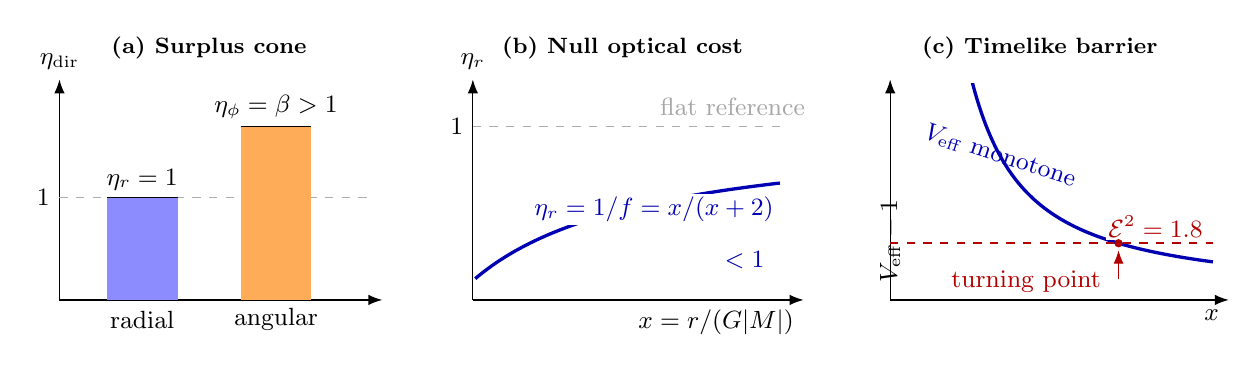
\begin{tikzpicture}[
  font=\small,
  >=Latex,
  axis/.style={->,line width=0.45pt},
  guide/.style={gray!65,dashed},
  curve/.style={blue!70!black,very thick}
]
% (a) Directional costs of a surplus cone.
\begin{scope}
  \node[font=\bfseries\footnotesize] at (2.15,3.55) {(a) Surplus cone};
  \draw[axis] (0.25,0.35) -- (4.35,0.35);
  \draw[axis] (0.25,0.35) -- (0.25,3.15)
    node[above] {$\eta_{\rm dir}$};
  \draw[guide] (0.25,1.65) -- (4.15,1.65);
  \node[left] at (0.25,1.65) {$1$};
  \fill[blue!45] (0.85,0.35) rectangle (1.75,1.65);
  \fill[orange!65] (2.55,0.35) rectangle (3.45,2.55);
  \draw (0.85,1.65) -- (1.75,1.65);
  \draw (2.55,2.55) -- (3.45,2.55);
  \node at (1.30,0.10) {radial};
  \node at (3.00,0.10) {angular};
  \node at (1.30,1.88) {$\eta_r=1$};
  \node at (3.00,2.80) {$\eta_\phi=\beta>1$};
\end{scope}

% (b) Radial null cost in the negative-mass exterior.
\begin{scope}[xshift=5.25cm]
  \node[font=\bfseries\footnotesize] at (2.15,3.55) {(b) Null optical cost};
  \draw[axis] (0.25,0.35) -- (4.45,0.35)
    node[below left] {$x=r/(G|M|)$};
  \draw[axis] (0.25,0.35) -- (0.25,3.15)
    node[above] {$\eta_r$};
  \draw[guide] (0.25,2.55) -- (4.25,2.55);
  \node[left] at (0.25,2.55) {$1$};
  \node[gray!70] at (3.55,2.80) {flat reference};
  \draw[curve,domain=0.28:4.15,samples=90,smooth]
    plot (\x,{0.35+2.2*\x/(\x+2)});
  \node[blue!70!black,fill=white,inner sep=1pt] at (2.55,1.50)
    {$\eta_r=1/f=x/(x+2)$};
  \node[blue!70!black] at (3.70,0.85) {$<1$};
\end{scope}

% (c) Timelike barrier for finite specific energy.
\begin{scope}[xshift=10.55cm]
  \node[font=\bfseries\footnotesize] at (2.15,3.55) {(c) Timelike barrier};
  \draw[axis] (0.25,0.35) -- (4.55,0.35)
    node[below left] {$x$};
  \draw[axis] (0.25,0.35) -- (0.25,3.15)
    node[midway,left,rotate=90] {$V_{\eff}-1$};
  \begin{scope}
    \clip (0.25,0.35) rectangle (4.40,3.10);
    \draw[curve,domain=0.72:4.35,samples=110,smooth]
      plot (\x,{0.35+0.9*((1+2/\x)*(1+1/(\x*\x))-1)});
    \draw[red!70!black,thick,dashed] (0.25,1.07) -- (4.35,1.07);
  \end{scope}
  \node[red!70!black,fill=white,inner sep=1pt] at (3.62,1.28)
    {$\mathcal E^2=1.8$};
  \fill[red!70!black] (3.15,1.07) circle (1.5pt);
  \draw[red!70!black,->] (3.15,0.62) -- (3.15,0.98);
  \node[red!70!black,anchor=east] at (3.05,0.58) {turning point};
  \node[blue!70!black,rotate=-18] at (1.65,2.18)
    {$V_{\eff}$ monotone};
\end{scope}
\end{tikzpicture}
\caption{Three operationally different effects.  (a) For a surplus cone with
$N=1$, radial optical cost is unchanged while angular cost is enlarged:
negative curvature does not mean less to traverse.  (b) In the negative-mass
Schwarzschild exterior, $x=r/(G|M|)$ and the radial null cost
$\eta_r=1/f=x/(x+2)$ lies below the flat reference.  (c) For specific angular
momentum $\ell/(G|M|)=1$, the timelike effective potential decreases
monotonically toward unity; finite specific energy produces a turning point
rather than a circular orbit.  The panels display intrinsic cost functions,
not embedding diagrams.}
\label{fig:costcomparison}
\end{figure*}

It is not, however, a statement about the four-volume density.  On a static
slice,
\begin{equation}
 \dd V_3=\frac{r^2\sin\theta}{\sqrt f}
 \dd r\,\dd\theta\,\dd\phi,
 \label{eq:spatialvolume}
\end{equation}
which is smaller than the flat value at the same areal radius.  This comparison
is geometric rather than a radial-coordinate convention: $r$ is fixed by the
area $4\pi r^2$ of each symmetry sphere.  The spacetime volume form is
\begin{equation}
 \dd V_4=N\,\dd t\,\dd V_3
 =r^2\sin\theta\,
 \dd t\,\dd r\,\dd\theta\,\dd\phi,
 \label{eq:fourvolume}
\end{equation}
exactly the flat expression in these geometrically fixed coordinates.  The
cancellation $N\sqrt{h}=r^2\sin\theta$ is specific to the Schwarzschild-form
metric in areal coordinates; it is not a general relation between repulsion
and four-volume.  The advance is controlled by $h_{ij}/N^2$, not by
$\sqrt{-g}$.

For impact parameter $b\gg G|M|$, the weak deflection is
\begin{equation}
 \delta\phi=-\frac{4G|M|}{b}
 +O\!\left(\frac{G^2M^2}{b^2}\right),
 \label{eq:deflection}
\end{equation}
so rays are divergently deflected and a background source is demagnified in
the weak-lensing regime.  The leading Shapiro contribution also changes sign,
\begin{equation}
 \Delta t=-2G|M|\ln\!\left(\frac{4r_er_o}{b^2}\right)
 +O(M^2),
 \label{eq:shapiroadvance}
\end{equation}
relative to a Minkowski filling with the same emitter and receiver areal radii,
the same impact-parameter convention, and the same asymptotic time
normalization.  This gives $E_U<0$ in the null channel.  These are statements
about the relevant optical congruence; full
spacetime focusing remains governed by the null Raychaudhuri equation, with
Ricci, Weyl, shear, and vorticity contributions \cite{wald-1984}.

With flat-space subtraction, the Brown--York energy of a round sphere is
\begin{equation}
 E_{\BY}(r)=\frac{r}{G}\left(1-\sqrt{f(r)}\right)<0,
 \label{eq:brown-york}
\end{equation}
consistent with quasilocal depletion relative to the reference
\cite{brown-york-1993}.  Its numerical value is subtraction dependent and it
is not a local energy density.  The minimal construction also has negative
Arnowitt--Deser--Misner (ADM) mass.
A distant compensating positive shell can change the exterior asymptotics and
total mass while leaving a negative quasilocal region, but its junctions and
stability must be analyzed as part of the enlarged model.

The shell should therefore be read as an effective exotic source, not as an
ordinary material proposal.  Quantum inequalities constrain weighted negative
energy densities for specified quantum fields and states
\cite{ford-roman-1995}; they do not automatically apply to an unspecified
classical shell.  Applying them here would require a concrete quantum source,
sampling worldline, and sampling function.

\section{Deletion is not a shortcut}
\label{sec:connectivity}

The distinction between cost and connectivity follows from one variational
observation.  Write an earliest-arrival problem abstractly as
\begin{equation}
 \mathcal T[\mathcal C,L]
 =\inf_{\gamma\in\mathcal C}\int_{\gamma}L,
 \label{eq:abstractcost}
\end{equation}
where $\mathcal C$ is the set of admissible paths and $L$ is their local cost.
There are then two independent ways to obtain an advance:
\begin{enumerate}
 \item lower $L$ on some existing paths, as a metric or lapse change does;
 \item enlarge $\mathcal C$, as a bridge or identification can do.
\end{enumerate}

Deleting a closed region while keeping the surrounding geometry fixed does
the opposite of the second operation: $\mathcal C'\subseteq\mathcal C$.
The comparison assumes that $L$ is held pointwise fixed on every surviving
path.  Therefore
\begin{equation}
 \mathcal T[\mathcal C',L]\geq
 \mathcal T[\mathcal C,L].
 \label{eq:deletionmonotonicity}
\end{equation}
For an ordinary length space this is the familiar inequality
$d_{Y\setminus H}(p,q)\geq d_Y(p,q)$.  In a fixed spacetime, excision can cause
detour, delay, scattering, disconnection, or no change, but not an earlier
arrival.  If removing matter changes the metric, the cost $L$ has changed and
the monotonicity statement no longer compares the same problem; this includes
the physically common case in which matter removal changes $h_{ij}$ or $N$.

Collapsing the boundary of an excised disk to a zero-cost point is not a
surplus cone; it creates a pinched quotient.  A physical bridge must have a
nonzero throat geometry, a causal orientation, and a stress tensor.  It must
also be checked for non-Hausdorff behavior and closed causal curves.  Under
the hypotheses of topological censorship, asymptotic flatness, global causal
conditions, and averaged null energy restrict observable nontrivial topology
\cite{friedman-schleich-witt-1993}; these hypotheses should be stated rather
than invoked as a slogan.  Traversable wormhole models accordingly constitute
a separate connectivity sector \cite{visser-1995}.

\section{If ``stuff'' is microscopic}
\label{sec:microscopic}

A literal constituent interpretation requires an additional microscopic law.
For example, causal-set models distinguish causal order from local finiteness
and element count \cite{bombelli-lee-meyer-sorkin-1987}.  Even in such a model,
fewer elements in a tube does not by itself imply earlier arrival: the order
relations determine which chains exist, the count represents a volume-like
quantity, and the dynamics must relate both to an effective metric.  Thinning
can reduce a count while also destroying routes.  The continuum boundary
kernel \eqref{eq:kernel} is therefore a target observable that a microscopic
model must reproduce, rather than something fixed by constituent density
alone.

Kleinert's second-gradient and nematic world-crystal models go further by
proposing mechanisms through which Einstein-like long-range dynamics might
emerge \cite{kleinert-1987,kleinert-2004}.  These constructions require special
constitutive or phase assumptions and therefore do not derive relativistic
dynamics from defect kinematics alone.  Moreover, a signed continuum defect
density can discard neutral defect populations and their higher correlations
\cite{kroner-2001}.

The same warning applies to defect ensembles.  A regularized two-dimensional
collection of cone defects has the signed curvature measure
\begin{equation}
 \Omega=\sum_i\alpha_i\delta_{p_i},
 \qquad \alpha_i=2\pi(1-\beta_i),
 \label{eq:defectmeasure}
\end{equation}
and a coarse-grained density in a window of area $A_{\Lambda}$,
\begin{equation}
 \overline K(\Lambda)
 =\frac{1}{A_{\Lambda}}
 \mathbb E\!\left[\sum_{p_i\in A_{\Lambda}}\alpha_i\right].
 \label{eq:coarsecurvature}
\end{equation}
This is meaningful as a two-dimensional or Regge-like curvature proxy.  It is
not a four-dimensional Ricci scalar and does not determine an optical cost.
The traversal observable must be coarse-grained separately, for example
\begin{equation}
 \overline E_a(\Lambda)
 =\mathbb E_{\mathcal P_{\Lambda}}
 \left[E_{U,a}(b_1,b_2)\right],
 \label{eq:coarsekernel}
\end{equation}
with the ensemble of boundary pairs $\mathcal P_{\Lambda}$ and probe channel
$a$ explicitly specified.  In particular,
$\overline K(\Lambda)=0$ does not imply
$\overline E_a(\Lambda)=0$: optical length depends nonlinearly on the metric
and on path minimization.  The sign of $\overline E_a$ must be calculated for
the specified ensemble rather than inferred from average defect charge.

Hausdorff and spectral dimensions can diagnose anomalous scaling, but they are
not signed curvature measures.  In a smooth $d$-dimensional geometry the heat
trace has the schematic small-$t$ form
\begin{equation}
 \operatorname{Tr}e^{t\Delta}
 \sim(4\pi t)^{-d/2}\left(a_0+a_1t+a_2t^2+\cdots\right),
 \label{eq:heattrace}
\end{equation}
where dimension appears in the leading exponent while curvature appears in
subleading coefficients such as $a_1$ \cite{vassilevich-2003}.  A running
spectral exponent is useful evidence for a nonclassical regime, but its excess
or deficit cannot be identified with the sign of scalar curvature without a
specific model and limiting theorem.

\section{Coarse-grained universality and local flatness}
\label{sec:universality}

Three scales should remain distinct: probe wavelength $\lambda_{\rm probe}$,
laboratory size $L_{\rm lab}$, and coarse-graining scale $\Lambda_{\rm cg}$.
They serve different purposes and need not obey one universal ordering.  A
fine wave can resolve and scatter from a defect even when a larger-scale
average looks smooth.  At a regular point $p$, a local inertial description
requires, schematically,
\begin{equation}
 L_{\rm lab}\ll\operatorname{dist}(p,H),
 \qquad
 L_{\rm lab}^2\|\operatorname{Riem}[g_{\eff}](p)\|\ll1,
 \label{eq:localflatness}
\end{equation}
where $H$ denotes unresolved singular cores.  A traversal curve approaching
the reference value at short scale is not by itself an equivalence-principle
theorem.

Before an effective response is called geometry, freely propagating species
should share a causal cone.  In a window
$\epsilon\ll\lambda_{\rm probe}\ll L_{\rm var}$, where $\epsilon$ is a
microscopic resolution scale and $L_{\rm var}$ is the shortest relevant
background-variation scale, a useful high-frequency criterion is
\begin{equation}
 P_a(x,k)=Z_a(x)g_{\eff}^{\mu\nu}(x)k_{\mu}k_{\nu},
 \qquad Z_a(x)>0,
 \label{eq:universality}
\end{equation}
for the principal symbol of every probe species $a$.  Species-dependent cones,
birefringence, or strong frequency dependence indicate an analogue medium
rather than one universal spacetime metric.  More concretely, after
nongravitational propagation delays have been removed, opposite signs of
$E_{U,a}$ for two minimally coupled massless probes in the same
high-frequency window rule out a single nondispersive effective metric for
those probes.  Outside that regime, differing signs need not be a geometric
falsifier.

The four sectors in Table~\ref{tab:fourquestions} can then be tested
independently:
\begin{enumerate}
 \item circumference and triangle data test angle defect and spatial curvature;
 \item released test bodies and clock comparisons test lapse gradients;
 \item boundary timing over directions, frequencies, and species tests
       traversal cost;
 \item path multiplicity and causal routing test connectivity.
\end{enumerate}
Agreement of these probes with one effective metric is a result to be
demonstrated, not an assumption contained in the word ``hole.''

For operational closure, any future claim of a spacetime hole should therefore
state six items: the reference filling and boundary identification, the probe
channel and frequency window, the measured kernel $E_{U,a}$, the lapse-gradient
response of released bodies and clocks, the angle or holonomy data, and the
admissible connectivity.  This checklist prevents one sector from being used
as unreported evidence for another.

\section{Discussion: measurement protocols and scales}
\label{sec:discussion}

The word \emph{observer} in this analysis denotes several measurement
protocols, not four independent geometries.  A freely falling local laboratory
tests the local light cone and tidal corrections to inertial motion.  Static
observers compare clock rates and measure the acceleration required to remain
at fixed position; Eq.~\eqref{eq:staticacc} gives coordinate components of that
acceleration, not a new scalar traversal cost.  A boundary signal network
measures the global kernel $E_U$ by recording emission and reception times.
The Brown--York quantity in Eq.~\eqref{eq:brown-york} is different again: it is
a quasilocal functional of a closed two-surface with a specified subtraction,
not a local energy density.  These protocols can be implemented by overlapping
sets of observers, but their outputs answer different questions.

The examples deliberately cross, rather than occupy, single rows of
Table~\ref{tab:fourquestions}.  The surplus cone changes angle and transverse
optical cost while leaving the radial optical cost, the ordinary radial force,
and the connectivity unchanged.  The negative-mass shell changes the lapse,
free fall, and null and timelike traversal costs while retaining the topology
of the reference construction.  Thus the four-sector table is a reporting
discipline, not a one-to-one assignment of models or observers to rows.

The scale requirements are likewise logically separate.  The window
$\epsilon\ll\lambda_{\rm probe}\ll L_{\rm var}$ supports an effective
continuum and a geometric-optics approximation, whereas
Eq.~\eqref{eq:localflatness} controls the size of a locally inertial
laboratory.  The coarse-graining scale $\Lambda_{\rm cg}$ must be specified by
the microscopic model; there is no universal hierarchy that fixes its order
relative to $L_{\rm lab}$ in every experiment.  In particular, the contrast
between the null advance and the timelike barrier of the shell is governed by
the access condition~\eqref{eq:accesscondition}, not by a wavelength
hierarchy.

Finally, the relative observables do not all use interchangeable reference
structures.  The kernel $E_U$ uses the filling and boundary identification
$(U_0,\iota)$; the directional optical ratio requires a specified local
comparison; the weak Shapiro advance uses the stated Minkowski comparator; and
the Brown--York energy uses its own surface subtraction.  Making each reference
explicit is what makes the reported sign meaningful and reproducible.

\section{Conclusion}
\label{sec:conclusion}

The intuition of less spacetime to traverse is viable when translated into a
reference-relative path cost.  In a static spacetime the translation is exact:
light measures the optical metric $h_{ij}/N^2$, and the boundary kernel
$E_U$ records delay or advance.  Volume density, curvature, force, and
connectivity provide other information but do not substitute for this cost.

The examples make the distinctions concrete.  A surplus cone has negative
curvature and enhanced transverse length but neither reduced radial cost nor a
force.  A repulsive negative-mass shell instead contracts the optical metric
and advances light while presenting an energy barrier to inward-moving massive
particles.  It requires exotic surface stress, so it is an exact effective
model rather than an ordinary source.  Deleting a region with unchanged cost
cannot create a shortcut; an advance requires a reduced metric cost or an
enlarged path set.  Any microscopic account of spacetime ``stuff'' must explain
how its constituent density and connectivity produce these operational
observables and why different probes see the same emergent geometry.

\begin{acknowledgments}
This research was funded in whole or in part by the \textit{Austrian Science
Fund (FWF)}.  Grant digital object identifier (DOI):
\url{https://doi.org/10.55776/PIN5424624}.
The author acknowledges TU Wien Bibliothek for financial support through its
Open Access Funding Programme.

OpenAI Codex was used to assist with manuscript criticism, literature
organization, derivation checks, and editorial revision.  The author directed
its use, independently verified the mathematical arguments and cited sources,
revised the resulting text, and assumes full responsibility for the
manuscript.
\end{acknowledgments}

% Portable bibliography: a subset copied from the user's master database plus
% the DOI-verified additions used in this manuscript.
\bibliography{svozil}

\end{document}
